\subsection{Цель выполнения лабораторной работы}\label{blockN.VariantM}
\textbf{Цель выполнения лабораторной работы }-- \GoalOfResearch

%-------------------------------------------------
\subsection{Задание}

Решить с помощью МКЭ уравнение \ref{usl}
\begin{align}\label{usl}
{{ a_int }}\frac{d^2u}{dx^2}  -{{ b_abs }} \frac{du}{dx}   +{{ b_abs }} \frac{du}{dx}   -{{ c_abs }}u   +{{ c_abs }}u   -{{ d_abs }}   +{{ d_abs }} 
=0,
\end{align}
при следующих граничных условиях (г. у.): 
\begin{align}\label{2_rod}
    u'(x={{ min_int_int }}) = {{ min_value_int }},
\end{align}
\begin{align}\label{1_rod}
    u'(x={{ max_int_int }}) = {{ max_value_int }}.
\end{align}

Количество конечных элементов
\begin{itemize}
    \item для первого расчета -- 20,
    \item для второго -- 40.
\end{itemize}

Также необходимо:
\begin{enumerate}
    \item Сравнить результаты с аналитическим решением. Оценить максимальную погрешность.
    \item Определить количество линейных КЭ, обеспечивающих такую же точность как и кубические.
\end{enumerate}

%-------------------------------------------------
\newpage
\subsection{Аналитическое решение}

На рисунке \ref{analit} представлено аналитическое решение поставленной задачи.
\begin{figure}[!h]
\begin{center}
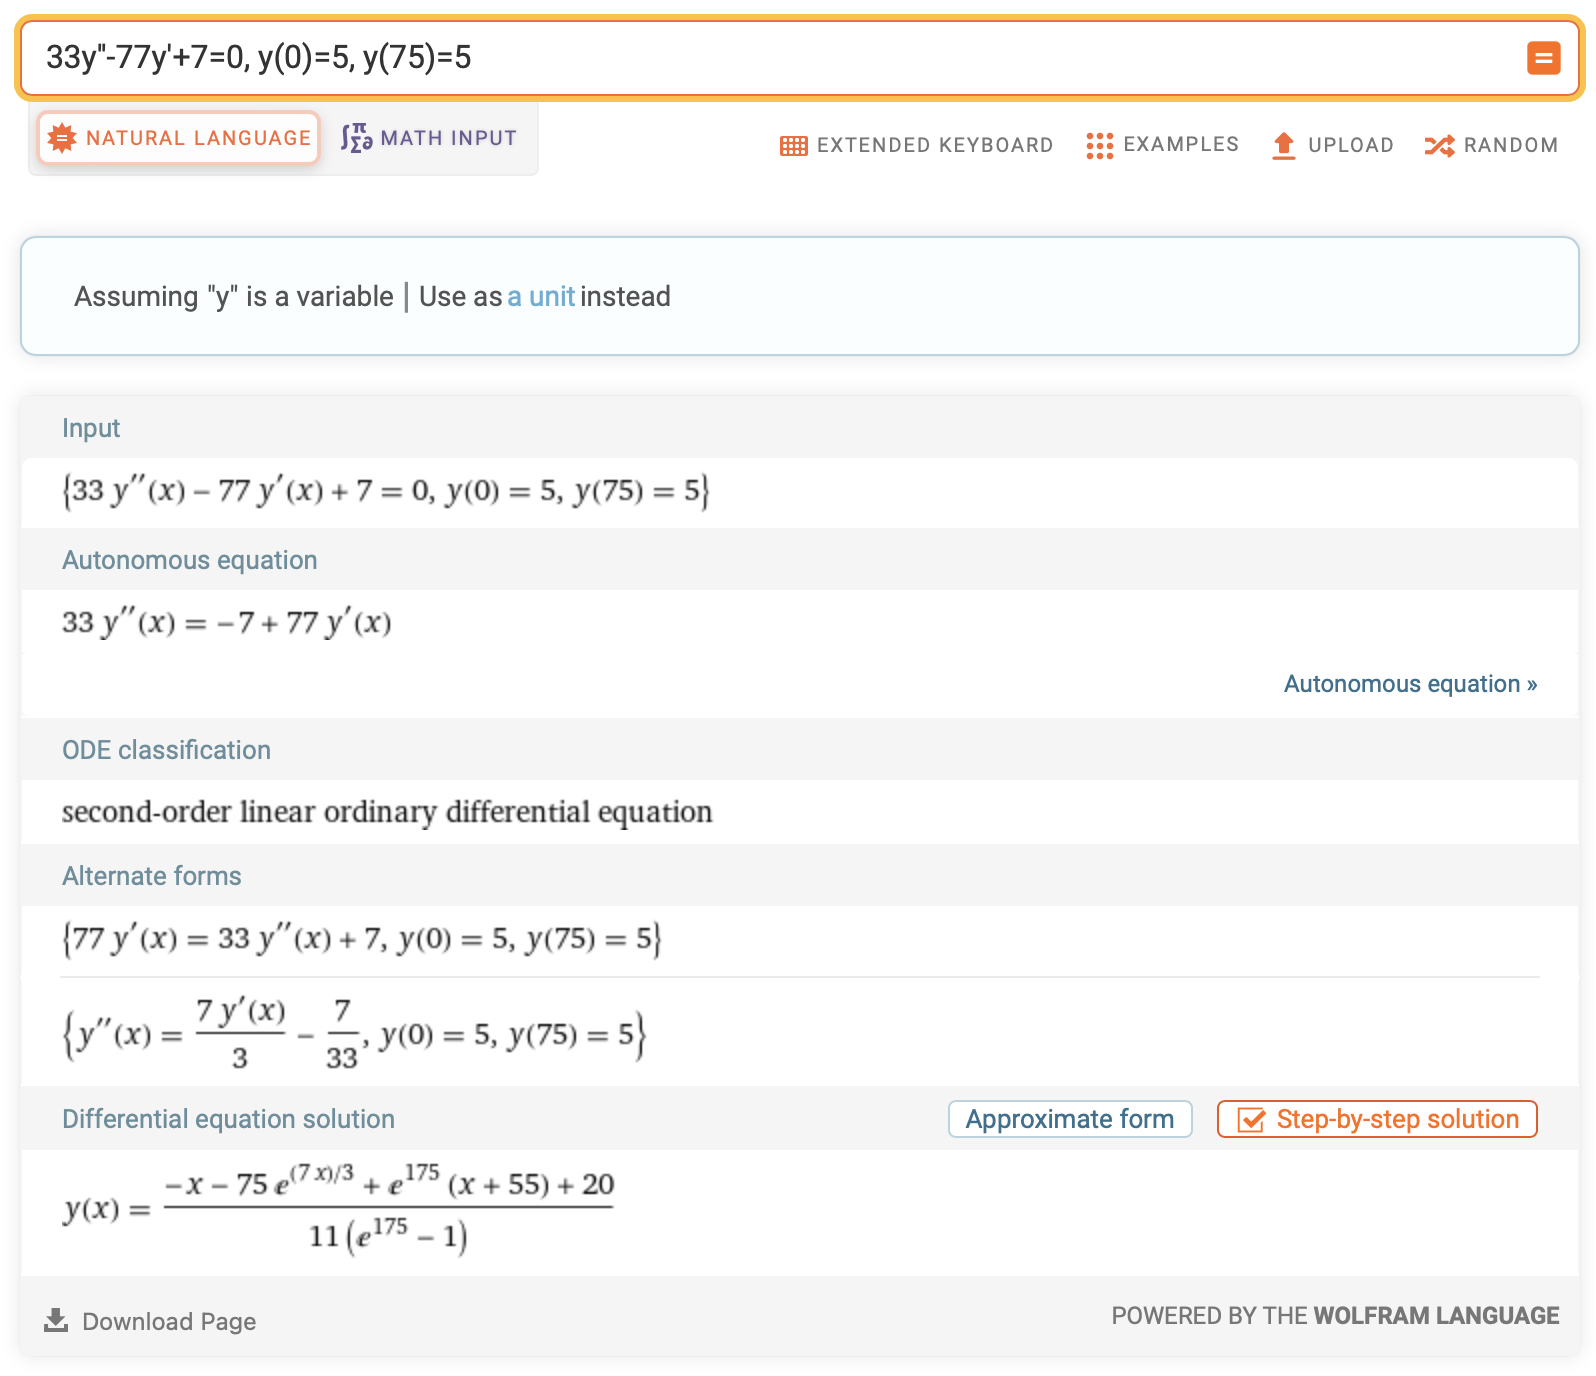
\includegraphics[scale = 0.5]{labs/img/img1}
\end{center}
\caption{Аналитическое решение}
\label{analit}
\end{figure}

Таким образом, получаем:
$$
u(x)={{ analytical_solution }}.
$$


\subsection{Получение локальных матрицы жесткости и вектора нагрузок}

Составим локальные матрицу жесткости и вектор нагрузок для уравнения \ref{usl}.

\subsubsection{Линейная функция-формы КЭ}

$$
\mathbf{u}=\begin{bmatrix}
(1-\frac{x}{L}) ; & \frac{x}{L}
\end{bmatrix}
\begin{bmatrix}
u_i \\
u_j
\end{bmatrix}
=\mathbf{N_eU},
$$
где $\mathbf{N_e}$ -- вектор функции формы конечного элемента (в данном случае линейной), его составляющие элементы - глобальные базисные функции, отличные от нуля в пределах этого элемента, $L$ -- длина КЭ.

В соответствии с методом Галеркина для уравнения \ref{usl}:
\begin{equation}\label{lin}
\int_0^L \mathbf{W_e}\left( {{ a_int }}\frac{d^2\mathbf{u}}{dx^2} -{{ b_abs }}   +{{ b_abs }} \frac{d\mathbf{u}}{dx}  -{{ c_abs }}u   +{{ c_abs }}u   -{{ d_abs }}   +{{ d_abs }} \right) d x=0,
\end{equation}
где $\mathbf{W_e=N_e}^T$.

$$\int_0^L \mathbf{W_e}\left({{ a_int }}\frac{d^2\mathbf{u}}{dx^2} -{{ b_abs }}   +{{ b_abs }} \frac{du}{dx}  -{{ c_abs }}u   +{{ c_abs }}u   -{{ d_abs }}   +{{ d_abs }} \right) d x = {{ a_int }}\int_0^L \mathbf{W_e} \frac{d^2 \mathbf{u}}{dx^2} dx  -{{ b_abs }} \int_0^L \mathbf{W_e}\frac{d\mathbf{u}}{dx} d x   +{{ b_abs }} \int_0^L \mathbf{W_e}\frac{d\mathbf{u}}{dx} d x   -{{ c_abs }} \int_0^L \mathbf{W_e u} d x   +{{ c_abs }} \int_0^L \mathbf{W_e u} dx   -{{ d_abs }} \int_0^L \mathbf{W_e}   +{{ d_abs }} \int_0^L \mathbf{W_e u} =0$$

Распишем каждое слагаемое отдельно:

$$
{{ a_int }}\int_0^L \mathbf{W_e} \frac{d^2 \mathbf{u}}{dx^2} dx={{ a_int }}\int_0^L
	\begin{bmatrix}
	(1-\frac{x}{L}) \\
	\frac{x}{L}
	\end{bmatrix}
\frac{d^2 \mathbf{u}}{dx^2} dx =
{{ a_int }}
	\begin{bmatrix}
	(1-\frac{x}{L}) \\
	\frac{x}{L}
	\end{bmatrix}
\frac{d\mathbf{u}}{dx} |_0^L -
$$
$$
 +{{ a_abs }}   -{{ a_abs }}  \int_0^L
\frac{d}{dx}
	\begin{bmatrix}
	(1-\frac{x}{L}) \\
	\frac{x}{L}
	\end{bmatrix}
\frac{d}{dx}
	\begin{bmatrix}
	(1-\frac{x}{L}); & \frac{x}{L}
	\end{bmatrix}
	\begin{bmatrix}
	u_i \\
	u_j
	\end{bmatrix}
=
	\begin{bmatrix}
	 +{{ a_abs }}   -{{ a_abs }} \frac{d\mathbf{u}}{dx}|_i \\
{{ a_int }}\frac{d\mathbf{u}}{dx}|_j
	\end{bmatrix}  +{{ a_abs }}   -{{ a_abs }} 
\begin{bmatrix}
\frac{1}{L}, & -\frac{1}{L} \\
-\frac{1}{L}, & \frac{1}{L}
\end{bmatrix}
\begin{bmatrix}
u_i \\
u_j
\end{bmatrix}
$$



$$
 -{{ b_abs }}   +{{ b_abs }} \int_0^L \mathbf{W_e} \frac{d \mathbf{u}}{dx} dx= -{{ b_abs }}   +{{ b_abs }} \int_0^L
	\begin{bmatrix}
	(1-\frac{x}{L}) \\
	\frac{x}{L}
	\end{bmatrix}
\frac{d \mathbf{u}}{dx}
	\begin{bmatrix}
	u_i \\
	u_j
	\end{bmatrix}
dx
=
$$
$$
= -\frac{ {{ b_abs }} }{L}   \frac{ {{ b_abs }} }{L} 
\int_0^L
\begin{bmatrix}
	(1-\frac{x}{L}) & (-1+\frac{x}{L})\\
	-\frac{x}{L} & \frac{x}{L}
\end{bmatrix}
\begin{bmatrix}
	u_i \\
	u_j
\end{bmatrix}
=
 -{{ b_abs }}   {{ b_abs }} 
\begin{bmatrix}
-\frac{1}{2}, & \frac{1}{2} \\
-\frac{1}{2}, & \frac{1}{2}
\end{bmatrix}
\begin{bmatrix}
u_i \\
u_j
\end{bmatrix}
$$



$$
 -{{ c_abs }}   {{ c_abs }} 
\int_0^L \mathbf{W_e} \mathbf{u} dx=
 -{{ c_abs }}   {{ c_abs }} 
\int_0^L
\begin{bmatrix}
	(1-\frac{x}{L}) \\
	\frac{x}{L}
\end{bmatrix}
\mathbf{u}
\begin{bmatrix}
	u_i \\
	u_j
\end{bmatrix}
dx
=
 -{{ c_abs }}   {{ c_abs }} 
\begin{bmatrix}
\frac{L}{3}, & \frac{L}{6} \\
\frac{L}{6}, & \frac{L}{3}
\end{bmatrix}
\begin{bmatrix}
u_i \\
u_j
\end{bmatrix}
$$



$$
{{ d_int }}\int_0^L \mathbf{W_e} d x= {{ d_int }}
\begin{bmatrix}
	\frac{L}{2} \\
	\frac{L}{2}
\end{bmatrix}
$$


Таким образом, для уравнения \ref{lin}, при использовании линейной функции-формы,  получаем (матмодель линейного КЭ):

$$
\begin{bmatrix}
	{{ a_int }}\frac{1}{L}  -{{ b_abs }} \frac{1}{2}   +{{ b_abs }} \frac{1}{2}  -{{ c_abs }} \frac{L}{3}   +{{ c_abs }} \frac{L}{3}, &  +{{ a_abs }}   -{{ a_abs }} \frac{1}{L}  +{{ b_abs }} \frac{1}{2}   -{{ b_abs }} \frac{1}{2}   -{{ c_abs }} \frac{L}{6}   +{{ c_abs }} \frac{L}{6} \\
	 +{{ a_abs }}   -{{ a_abs }}  \frac{1}{L}  -{{ b_abs }} \frac{1}{2}   +{{ b_abs }} \frac{1}{2}   -{{ c_abs }} \frac{L}{6}   +{{ c_abs }} \frac{L}{6}, &  {{ a_int }}\frac{1}{L}  +{{ b_abs }} \frac{1}{2}   -{{ b_abs }} \frac{1}{2}   -{{ c_abs }} \frac{L}{3}   +{{ c_abs }} \frac{L}{3}
\end{bmatrix}
\begin{bmatrix}
	u_i \\
	u_j
\end{bmatrix}=
\begin{bmatrix}
	 {{ a_abs }}   -{{ a_abs }} \frac{du}{dx}|_i  -{{ d_abs }} \frac{L}{2}   +{{ d_abs }} \frac{L}{2} \\
	{{ a_int }}\frac{du}{dx}|_j  -{{ d_abs }} \frac{L}{2}   +{{ d_abs }} \frac{L}{2} 
\end{bmatrix}
$$


\subsubsection{Кубическая функция-формы КЭ}
$$
\mathbf{u}=\begin{bmatrix}
-\frac{9x^3}{2L^3}+\frac{18x^2}{2L^2}-\frac{11x}{2L} + 1;
\frac{27x^3}{2L^3}-\frac{45x^2}{2L^2}+\frac{9x}{L};
-\frac{27x^3}{2L^3}+\frac{36x^2}{2L^2}-\frac{9x}{2L};
\frac{9x^3}{2L^3}-\frac{9x^2}{2L^2}-\frac{x}{L};
\end{bmatrix}
\begin{bmatrix}
u_i \\
u_j\\
u_k\\
u_l
\end{bmatrix}
=\mathbf{N_eU},
$$

Как и для линейной функции-формы применим метод Галеркина (см. уравнение \ref{lin}) и рассмотрим каждое слагаемое отдельно.

$${{ a_int }} \int_0^L \mathbf{W_e} \frac{d^2 \mathbf{u}}{dx^2} dx
=
{{ a_int }}\int_0^L
\begin{bmatrix}
	-\frac{9x^3}{2L^3}&+&\frac{18x^2}{2L^2}&-&\frac{11x}{2L} &+& 1\\
	\frac{27x^3}{2L^3}&-&\frac{45x^2}{2L^2}&+&\frac{9x}{L}&&\\
	-\frac{27x^3}{2L^3}&+&\frac{36x^2}{2L^2}&-&\frac{9x}{2L}&&\\
	\frac{9x^3}{2L^3}&-&\frac{9x^2}{2L^2}&-&\frac{x}{L}&&
\end{bmatrix}
\frac{d^2 \mathbf{u}}{dx^2} dx
=
$$
$$
=
{{ a_int }}
\begin{bmatrix}
	-\frac{9x^3}{2L^3}&+&\frac{18x^2}{2L^2}&-&\frac{11x}{2L} &+& 1\\
	\frac{27x^3}{2L^3}&-&\frac{45x^2}{2L^2}&+&\frac{9x}{L}&&\\
	-\frac{27x^3}{2L^3}&+&\frac{36x^2}{2L^2}&-&\frac{9x}{2L}&&\\
	\frac{9x^3}{2L^3}&-&\frac{9x^2}{2L^2}&-&\frac{x}{L}&&
\end{bmatrix}
\frac{d\mathbf{u}}{dx} |_0^L
 +{{ a_abs }}   -{{ a_abs }}  \int_0^L \frac{d}{dx}
\begin{bmatrix}
	-\frac{9x^3}{2L^3}&+&\frac{18x^2}{2L^2}&-&\frac{11x}{2L} &+& 1\\
	\frac{27x^3}{2L^3}&-&\frac{45x^2}{2L^2}&+&\frac{9x}{L}&&\\
	-\frac{27x^3}{2L^3}&+&\frac{36x^2}{2L^2}&-&\frac{9x}{2L}&&\\
	\frac{9x^3}{2L^3}&-&\frac{9x^2}{2L^2}&-&\frac{x}{L}&&
\end{bmatrix}
\frac{d}{dx} \mathbf{u}
=$$
$$
=
\begin{bmatrix}
	 +{{ a_abs }}   -{{ a_abs }} \frac{d\mathbf{u}}{dx}|_i \\
	0\\
	0\\
{{ a_int }}\frac{d\mathbf{u}}{dx}|_l
\end{bmatrix}
 +{{ a_abs }}   -{{ a_abs }} 
\begin{bmatrix}
\begin{array}{rrrr}
	\frac{37}{10L} & -\frac{189}{40} & \frac{27}{20L} & -\frac{13}{40L}\\
	-\frac{189}{40} & \frac{54}{5L} & -\frac{297}{40L} & \frac{27}{20L}\\
	\frac{27}{20L} &  -\frac{297}{40L} & \frac{54}{5L} & -\frac{189}{40}\\
	-\frac{13}{40L} & \frac{27}{20L} & -\frac{189}{40} & \frac{37}{10L}
\end{array}
\end{bmatrix}
\begin{bmatrix}
u_i \\
u_j \\
u_k\\
u_l
\end{bmatrix}
$$


$$
 -{{ b_abs }}   {{ b_abs }}  \int_0^L \mathbf{W_e} \frac{d \mathbf{u}}{dx} dx
=
 -{{ b_abs }}   {{ b_abs }} \int_0^L
\begin{bmatrix}
  -\frac{9x^3}{2L^3}&+&\frac{18x^2}{2L^2}&-&\frac{11x}{2L} &+& 1\\
  \frac{27x^3}{2L^3}&-&\frac{45x^2}{2L^2}&+&\frac{9x}{L}&&\\
  -\frac{27x^3}{2L^3}&+&\frac{36x^2}{2L^2}&-&\frac{9x}{2L}&&\\
  \frac{9x^3}{2L^3}&-&\frac{9x^2}{2L^2}&-&\frac{x}{L}&&
\end{bmatrix}
\frac{d \mathbf{u}}{dx} dx
=
$$
$$
=
 -{{ b_abs }}   {{ b_abs }} 
\begin{bmatrix}
\begin{array}{rrrr}
	-\frac{1}{2} & \frac{57}{80} & -\frac{3}{10} & \frac{7}{80}\\
	-\frac{57}{80} & 0 & \frac{81}{80} & -\frac{3}{10} \\
	\frac{3}{10} & -\frac{81}{80} & 0 & -\frac{3}{10}\\
	-\frac{7}{80} & \frac{3}{10} & -\frac{57}{80} & \frac{1}{2}
\end{array}
\end{bmatrix}
\begin{bmatrix}
	u_i \\
	u_j \\
	u_k\\
	u_l
\end{bmatrix}
$$



$$
 -{{ c_abs }}   {{ c_abs }}  \int_0^L \mathbf{W_e} \mathbf{u} dx
=
 -{{ c_abs }}   {{ c_abs }}  \int_0^L
\begin{bmatrix}
  -\frac{9x^3}{2L^3}&+&\frac{18x^2}{2L^2}&-&\frac{11x}{2L} &+& 1\\
  \frac{27x^3}{2L^3}&-&\frac{45x^2}{2L^2}&+&\frac{9x}{L}&&\\
  -\frac{27x^3}{2L^3}&+&\frac{36x^2}{2L^2}&-&\frac{9x}{2L}&&\\
  \frac{9x^3}{2L^3}&-&\frac{9x^2}{2L^2}&-&\frac{x}{L}&&
\end{bmatrix}
\mathbf{u} dx
=
$$
$$
=
 -{{ c_abs }}   {{ c_abs }} 
\begin{bmatrix}
\begin{array}{rrrr}
	\frac{8L}{105} 		&  \frac{33L}{560} & -\frac{3L}{140}  &  \frac{119L}{1680}\\
	\frac{33L}{560} 	&  \frac{27L}{170} & -\frac{27L}{560} & -\frac{3L}{140} \\
   -\frac{3L}{140} 		& -\frac{27L}{560} &  \frac{27L}{170} &  \frac{33L}{560} \\
    \frac{19L}{1680} 	& -\frac{3L}{140}  &  \frac{33L}{560} &  \frac{8L}{105}
\end{array}
\end{bmatrix}
\begin{bmatrix}
	u_i \\
	u_j \\
	u_k\\
	u_l
\end{bmatrix}
$$



$$
{{ d_int }} \int_0^L \mathbf{W_e} d x
=
{{ d_int }}
\begin{bmatrix}
	\frac{L}{8} \\
	\frac{3L}{8}\\
	\frac{3L}{8}\\
	\frac{L}{8}
\end{bmatrix}
$$


\newpage
Таким образом, для уравнения \ref{lin}, при использовании кубической функции-формы,  получаем:

$$
\begin{bmatrix}
		{{ a_int }}\frac{37}{10L}  -{{ b_abs }} \frac{1}{2}   +{{ b_abs }} \frac{1}{2}   -{{ c_abs }} \frac{8L}{105}   +{{ c_abs }} \frac{8L}{105}  &
		 +{{ a_abs }} \frac{189}{40L}   -{{ a_abs }} \frac{189}{40L}   +{{ b_abs }} \frac{57}{80}   -{{ b_abs }} \frac{57}{80}   -{{ c_abs }} \frac{33L}{560}   +{{ c_abs }} \frac{33L}{560}  &
		{{ a_int }}\frac{27}{20L} -{{ b_abs }} \frac{3}{10}   +{{ b_abs }} \frac{3}{10}   +{{ c_abs }} \frac{3L}{140}   -{{ c_abs }} \frac{3L}{140}  &
		 {{ a_abs }} \frac{13}{40L}   -{{ a_abs }} \frac{13}{40L}   +{{ b_abs }}\frac{7}{80}   -{{ b_abs }}\frac{7}{80}   -{{ c_abs }} \frac{119L}{1680}   +{{ c_abs }} \frac{119L}{1680} \\

		 {{ a_abs }}   -{{ a_abs }} \frac{189}{40L}  -{{ b_abs }}\frac{57}{80}   +{{ b_abs }}\frac{57}{80}   -{{ c_abs }} \frac{33L}{560}   +{{ c_abs }} \frac{33L}{560}  &
		{{ a_int }}\frac{54}{5L}+0  -{{ c_abs }} \frac{27L}{170}   +{{ c_abs }} \frac{27L}{170}  &
		 {{ a_abs }}   -{{ a_abs }} \frac{297}{40L} +{{ b_abs }}\frac{81}{80}   -{{ b_abs }}\frac{81}{80}   +{{ c_abs }} \frac{27L}{560}   -{{ c_abs }} \frac{27L}{560}  &
		{{ a_int }}\frac{27}{20L}  -{{ b_abs }} \frac{3}{10}   +{{ b_abs }}\frac{3}{10}   +{{ c_abs }} \frac{27L}{560}   -{{ c_abs }} \frac{27L}{560}  \\

		{{ a_int }}\frac{27}{20L}  +{{ b_abs }} \frac{3}{10}   -{{ b_abs }} \frac{3}{10}    +{{ c_abs }} \frac{27L}{560}   -{{ c_abs }} \frac{27L}{560}  &
		 +{{ a_abs }}   -{{ a_abs }} \frac{297}{40L} -{{ b_abs }} \frac{81}{80}   +{{ b_abs }} \frac{81}{80}   +{{ c_abs }} \frac{27L}{560}   -{{ c_abs }} \frac{27L}{560}  &
		{{ a_int }}\frac{54}{5L}+0  -{{ c_abs }} \frac{27L}{170}   +{{ c_abs }} \frac{27L}{170}  &
		 +{{ a_abs }}   -{{ a_abs }} \frac{189}{40L}  +{{ b_abs }} \frac{57}{80}   -{{ b_abs }} \frac{57}{80}   -{{ c_abs }} \frac{33L}{560}   +{{ c_abs }} \frac{33L}{560}  \\

	     {{ a_abs }}   -{{ a_abs }} \frac{13}{40L}  -{{ b_abs }} \frac{7}{80}   +{{ b_abs }} \frac{7}{80}   -{{ c_abs }} \frac{19L}{1680}   +{{ c_abs }} \frac{19L}{1680}  &
		{{ a_int }}\frac{27}{20L} +{{ b_abs }}   -{{ b_abs }} \frac{3}{10}  -{{ c_abs }} \frac{3L}{140}   +{{ c_abs }} \frac{3L}{140}  &
		 {{ a_abs }}   -{{ a_abs }} \frac{189}{40L} +{{ b_abs }}\frac{57}{80}   -{{ b_abs }}\frac{57}{80}   -{{ c_abs }} \frac{33L}{560}   +{{ c_abs }} \frac{33L}{560}  &
		{{ a_int }}\frac{37}{10L}  +{{ b_abs }}\frac{1}{2}   -{{ b_abs }}\frac{1}{2}   -{{ c_abs }} \frac{8L}{105}   +{{ c_abs }} \frac{8L}{105} 
\end{bmatrix}
\cdot
$$
\begin{align}\label{cub}
\cdot
\begin{bmatrix}
	u_i \\
	u_j \\
	u_k\\
	u_l
\end{bmatrix}
=
\begin{bmatrix}
     {{ d_int }}\frac{L}{8}   +{{ a_abs }} \frac{du}{dx}|_i   -{{ a_abs }} \frac{du}{dx}|_i   \\
	 {{ d_int }}\frac{3L}{8}  0 \\
	 {{ d_int }}\frac{3L}{8}  0 \\
	 {{ d_int }}\frac{L}{8}   -{{ a_abs }} \frac{du}{dx}|_l   +{{ a_abs }} \frac{du}{dx}|_l 
\end{bmatrix}
\end{align}

Локальные матрицу жесткости и вектор нагрузок из уравнения \ref{cub} с помощью матричных преобразований приведем к следующему виду:

$$ \begin{bmatrix}
a_{11}     &  0  & 0  &  a_{14}\\
a_{21}     &  a_{22}  & 0  &  a_{24}\\
a_{31}     &  0  &  a_{33} &  a_{34}\\
a_{41}     &  0  & 0  &  a_{44}
\end{bmatrix}
\begin{bmatrix}
u_i \\
u_j \\
u_k\\
u_l
\end{bmatrix} =
\begin{bmatrix}
b_1  +{{ a_abs }}   -{{ a_abs }}  \frac{du}{dx}|_i \\
b_2\\
b_3\\
b_4  -{{ a_abs }}   +{{ a_abs }}  \frac{du}{dx}|_l
\end{bmatrix}$$

Для упрощения расчетов преобразуем систему выше, исключив внутренние узлы. Таким образом СЛАУ (математическая модель кубического КЭ):

$$ \begin{bmatrix}
a_{11}     &   a_{14}\\
a_{41}     &    a_{44}
\end{bmatrix}
\begin{bmatrix}
u_i \\
u_l
\end{bmatrix} =
\begin{bmatrix}
b_1  +{{ a_abs }}   -{{ a_abs }}  \frac{du}{dx}|_i \\
b_4  -{{ a_abs }}   +{{ a_abs }}  \frac{du}{dx}|_l
\end{bmatrix}$$

%-------------------------------------------------
\subsection{Получение глобальных матрицы жесткости и вектора нагрузок}

Проведем процедуры ансамблирования и учет граничных условий для формирования итоговой математической модели.

\subsubsection{Ансамблирование}

Пусть локальные матрица жесткости и вектор неизвестных заданы следующим образом

$$
\begin{bmatrix}
a_{11}     &   a_{12}\\
a_{21}     &    a_{22}
\end{bmatrix}
\begin{bmatrix}
u_i \\
u_j
\end{bmatrix} =
\begin{bmatrix}
b_1  +{{ a_abs }}   -{{ a_abs }}  \frac{du}{dx}|_i \\
b_2  -{{ a_abs }}   +{{ a_abs }}  \frac{du}{dx}|_l
\end{bmatrix},$$

тогда, при разбитие области на $n$ КЭ, глобальная матрица жесткости  будет иметь размерность $(n+1)\cdot(n+1)$:

$$ \begin{bmatrix}
a_{11}^1     &   a_{12}^1         &   0 & \cdots & 0 & 0 & 0  & 0\\
a_{21}^1     &    a_{22}^1+a_{11}^2 & a_{12}^2  & 0 & \cdots & 0 & 0  & 0\\
0     &    a_{21}^2 & a_{22}^2+a_{11}^3  &  a_{12}^3  & 0 & \cdots & 0  & 0\\
0     &    0  & a_{21}^3  & a_{22}^3+ \cdots  &  & &   & 0\\
\vdots & \vdots & \vdots & \vdots &  &  &   & \vdots\\
0 & 0 & 0 & 0 &  0 & 0 & \cdots+a_{11}^n  & a_{12}^n\\
0 & 0 & 0 & 0 &  0 & 0 & a_{21}^n  & a_{22}^n
\end{bmatrix}
\begin{bmatrix}
u_0 \\
u_1 \\
u_2\\
u_3\\
\vdots\\
u_{n-1}\\
u_n
\end{bmatrix} =
\begin{bmatrix}
b_1^1  +{{ a_abs }}   -{{ a_abs }}  \frac{du}{dx}|_0 \\
b_2^1+b_1^2\\
b_2^2+b_1^3\\
b_2^3+b_1^4\\
\vdots\\
b_2^{n-1}+b_1^n\\
b_2^n  -{{ a_abs }}   +{{ a_abs }}  \frac{du}{dx}|_L
\end{bmatrix}
$$

\subsubsection{Учет граничных условий}

Применим граничные условия первого (см. \ref{1_rod}) и второго рода (см. \ref{2_rod}) к выведенной выше системе.

$$
\begin{bmatrix}
1     &   0        &   0 & \cdots & 0 & 0 & 0  & 0\\
a_{21}^1     &    a_{22}^1+a_{11}^2 & a_{12}^2  & 0 & \cdots & 0 & 0  & 0\\
0     &    a_{21}^2 & a_{22}^2+a_{11}^3  &  a_{12}^3  & 0 & \cdots & 0  & 0\\
0     &    0  & a_{21}^3  & a_{22}^3+ \cdots  &  & &   & 0\\
\vdots & \vdots & \vdots & \vdots &  &  &   & \vdots\\
0 & 0 & 0 & 0 &  0 & 0 & \cdots+a_{11}^n  & a_{12}^n\\
0 & 0 & 0 & 0 &  0 & 0 & 0 & 1
\end{bmatrix}
\begin{bmatrix}
u_0 \\
u_1 \\
u_2\\
u_3\\
\vdots\\
u_{n-1}\\
u_n
\end{bmatrix} =
\begin{bmatrix}
 {{min_value_int}}  b_1^1  +{{ a_abs }}   -{{ a_abs }}  \cdot {{ min_value_int }}   \\
b_2^1+b_1^2\\
b_2^2+b_1^3\\
b_2^3+b_1^4\\
\vdots\\
b_2^{n-1}+b_1^n\\
 {{max_value_int}}  b_2^n  -{{ a_abs }}   +{{ a_abs }}  \cdot {{ max_value_int }}   \\
\end{bmatrix}
$$

\subsection{Анализ результатов}

Проведем сравнение результатов согласно заданию.

\subsubsection{Линейная функция-формы}


На рисунках \ref{l_20}, \ref{l_40} представлены графики полученные с помощью МКЭ (линейная функция-формы).

\begin{figure}[!h]
    \centering
    \begin{minipage}{0.5\textwidth}
        \centering
        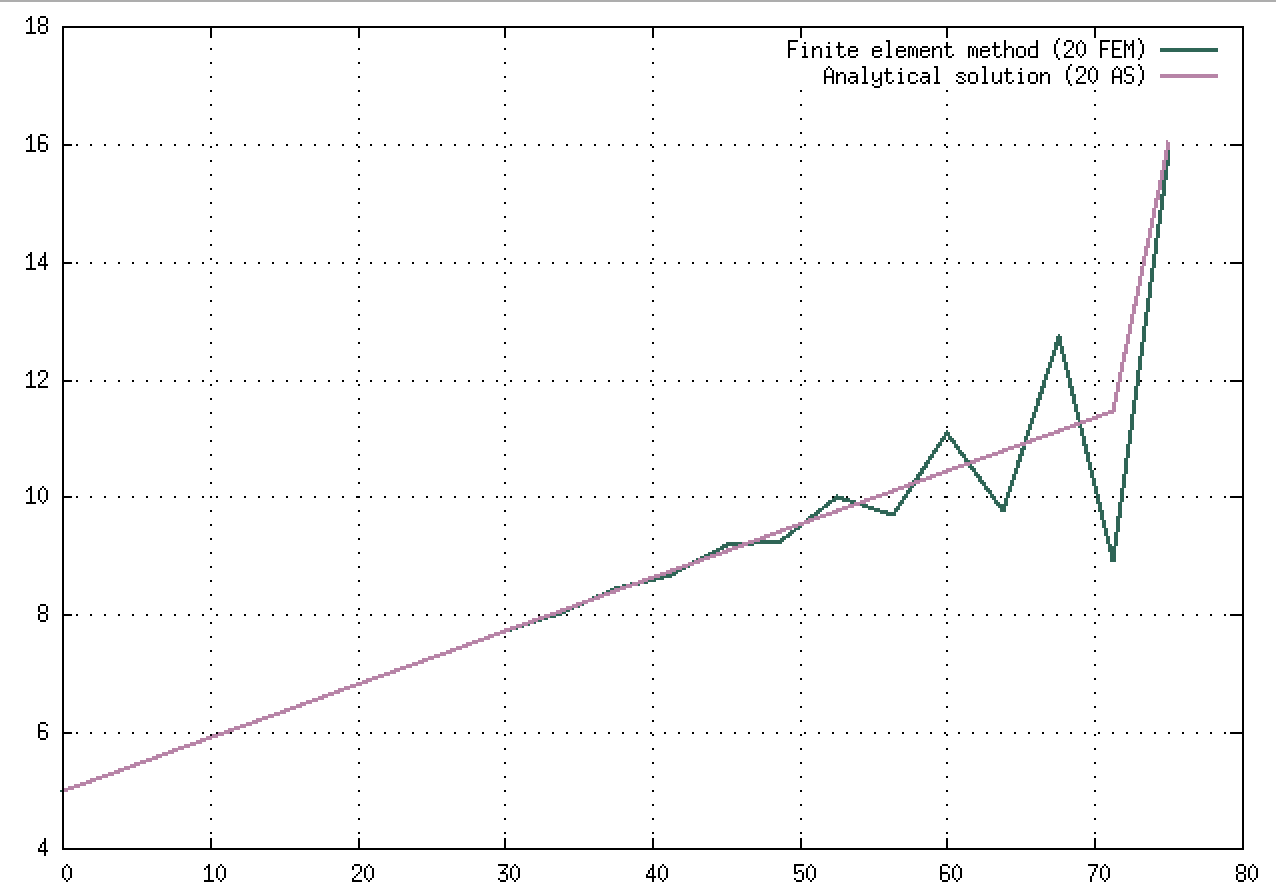
\includegraphics[width=1\textwidth]{labs/img/lin/20.png} % первое изображениие
        \caption{Результат работы программы для 20 КЭ}
        \label{l_20}
    \end{minipage}\hfill
    \begin{minipage}{0.5\textwidth}
        \centering
        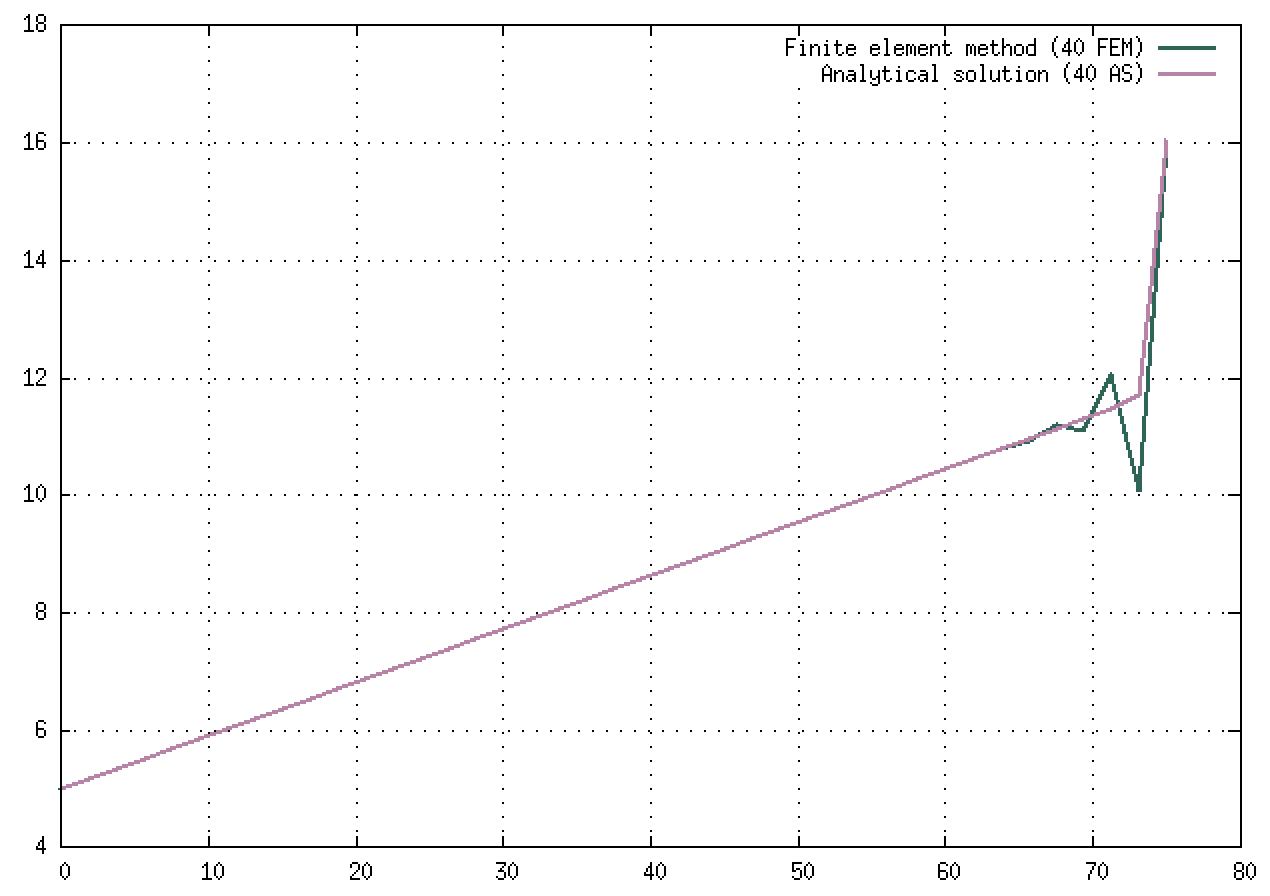
\includegraphics[width=1\textwidth]{labs/img/lin/40.png} % второе изображение
        \caption{Результат работы программы для 40 КЭ}
        \label{l_40}
    \end{minipage}
\end{figure}

\begin{table}[H]
\centering
\begin{tabular}{|c|c|c|c|}
\hline
X & Аналитическое & МКЭ-    & Абсолютная \\
  & решение       & решение & погрешность \\
\hline
\input{labs/text/tab/lin_20.txt} \\
\hline
\end{tabular}
\caption{20 линейных КЭ}
\label{table:lin_20}
\end{table}

\begin{table}[H]
\centering
\begin{tabular}{|c|c|c|c|}
\hline
X & Аналитическое & МКЭ-    & Абсолютная \\
  & решение       & решение & погрешность \\
\hline
\input{labs/text/tab/lin_40.txt} \\
\hline
\end{tabular}
\caption{40 линейных КЭ}
\label{table:lin_40}
\end{table}

Максимальная абсолютная погрешность \input{labs/text/pgr/lin_20.txt} и \input{labs/text/pgr/lin_40.txt} соответственно.

\subsubsection{Кубическая функция-формы}

На рисунках \ref{c_20}, \ref{c_40} представлены графики полученные с помощью МКЭ (кубическая функция-формы).

\begin{figure}[!h]
    \centering
    \begin{minipage}{0.5\textwidth}
        \centering
        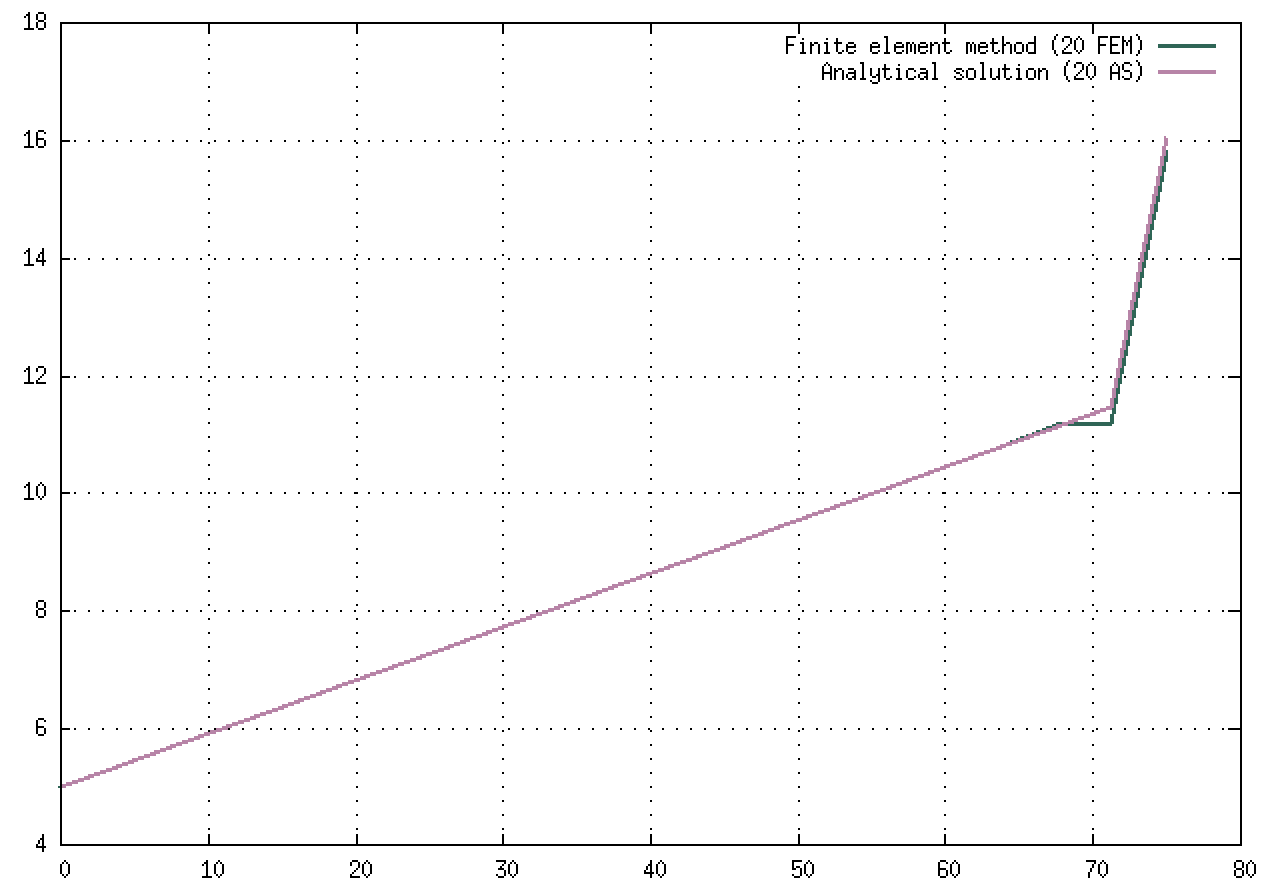
\includegraphics[width=1\textwidth]{labs/img/cub/20.png} % первое изображениие
        \caption{Результат работы программы для 20 КЭ}
        \label{c_20}
    \end{minipage}\hfill
    \begin{minipage}{0.5\textwidth}
        \centering
        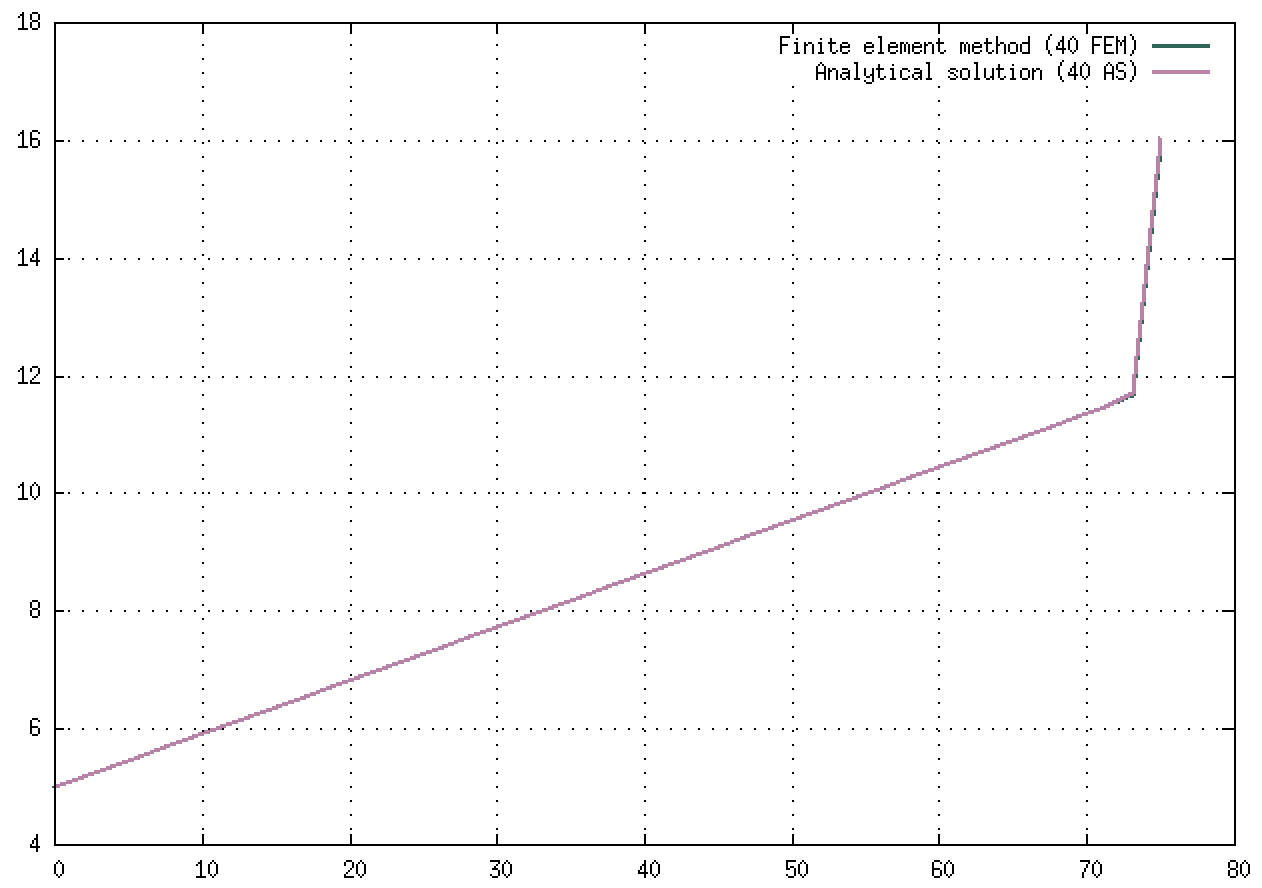
\includegraphics[width=1\textwidth]{labs/img/cub/40.png} % второе изображение
        \caption{Результат работы программы для 40 КЭ}
        \label{c_40}
    \end{minipage}
\end{figure}

\begin{table}[H]
\centering
\begin{tabular}{|c|c|c|c|}
\hline
X & Аналитическое & МКЭ-    & Абсолютная \\
  & решение       & решение & погрешность \\
\hline
\input{labs/text/tab/cub_20.txt} \\
\hline
\end{tabular}
\caption{20 кубических КЭ}
\label{table:lin_20}
\end{table}

\begin{table}[H]
\centering
\begin{tabular}{|c|c|c|c|}
\hline
X & Аналитическое & МКЭ-    & Абсолютная \\
  & решение       & решение & погрешность \\
\hline
\input{labs/text/tab/cub_40.txt} \\
\hline
\end{tabular}
\caption{40 кубических КЭ}
\label{table:lin_40}
\end{table}

Максимальная абсолютная погрешность \input{labs/text/pgr/cub_20.txt} и \input{labs/text/pgr/cub_40.txt} соответственно.


\subsubsection{Нахождение количества линейных КЭ, обеспечивающих ту же точность, что и 20 кубических}

Так как очевидно, что при увлечении числа КЭ точность растет, найдем искомое следуя алгоритму, представленному на рисунке \ref{alg}.

\begin{figure}[H]
\centerline{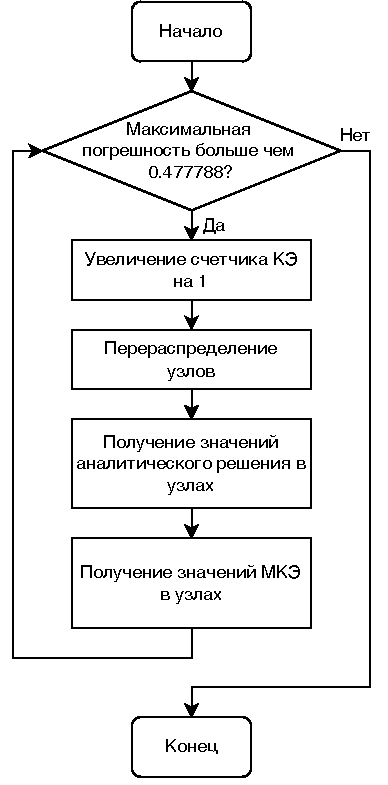
\includegraphics[scale = 0.65]{labs/img/img2.pdf}}
\caption{Алгоритм нахождения количества КЭ, заданную точность}
\label{alg}
\end{figure}

Реализовав данный алгоритм с начальным количеством КЭ=20 и увеличивая счетчик всегда на 1 получаем необходимое количество КЭ, равное \input{labs/text/pogr.txt}КЭ.

\subsection{Код}

\begin{lstlisting}[language=c++, label=prog,caption={\textit{Реализация МКЭ}}]

	{{ code }}

\end{lstlisting}
%-------------------------------------------------
\subsection{Вывод}

В ходе выполнения лабораторной работы был реализован МКЭ для различных функций форм, а также найдено количество линейных КЭ обеспечивающих точность 20ти кубических КЭ.

% --------------------------------------
% Атрибуты задачи
\labattributes{}{}{}{}{студент группы \EduGroup, \Author}{\Year, \Semestr}
%--------------

%  -{{ a_abs }}   +{{ a_abs }} 
%  +{{ a_abs }}   -{{ a_abs }} 

%  -{{ b_abs }}   +{{ b_abs }} 
%  +{{ b_abs }}   -{{ b_abs }} 

%  -{{ d_abs }}   +{{ d_abs }} 
%  +{{ d_abs }}   -{{ d_abs }} 